\documentclass[11pt,a4paper]{article}

% Packages
\usepackage[utf8]{inputenc}
\usepackage[T1]{fontenc}
\usepackage{lmodern}
\usepackage[margin=1in]{geometry}
\usepackage{hyperref}
\usepackage{listings}
\usepackage{xcolor}
\usepackage{graphicx}
\usepackage{tikz}
\usetikzlibrary{shapes,arrows,positioning,fit,calc,decorations.pathreplacing}
\usepackage{amsmath,amssymb}
\usepackage{booktabs}
\usepackage{enumitem}
\usepackage{fancyhdr}
\usepackage{tocloft}
\usepackage{tabularx}
\usepackage{multirow}
\usepackage{algorithm}
\usepackage{algpseudocode}

% Hyperref setup
\hypersetup{
    colorlinks=true,
    linkcolor=blue,
    filecolor=magenta,
    urlcolor=cyan,
}

% Code listing style
\definecolor{codebg}{RGB}{245,245,245}
\definecolor{codegreen}{RGB}{0,128,0}
\definecolor{codegray}{RGB}{128,128,128}
\definecolor{codepurple}{RGB}{128,0,128}
\definecolor{rustblue}{RGB}{0,122,204}

\lstdefinestyle{rustcode}{
    backgroundcolor=\color{codebg},
    basicstyle=\ttfamily\small,
    breakatwhitespace=false,
    breaklines=true,
    captionpos=b,
    commentstyle=\color{codegreen},
    keywordstyle=\color{rustblue}\bfseries,
    numberstyle=\tiny\color{codegray},
    stringstyle=\color{codepurple},
    showstringspaces=false,
    numbers=left,
    numbersep=5pt,
    frame=single,
    rulecolor=\color{black},
    tabsize=4,
    morekeywords={async,await,pub,fn,struct,impl,let,mut,if,else,match,loop,for,while,use,mod,Arc,Mutex,Duration}
}

\lstset{style=rustcode}

% Header/Footer
\pagestyle{fancy}
\fancyhf{}
\rhead{BetterSys Latency Analysis}
\lhead{Tick-to-Trade Performance}
\rfoot{Page \thepage}

% Title
\title{%
    \textbf{BetterSys: Tick-to-Trade Latency Analysis} \\
    \large Critical Path Decomposition, Distribution Measurement, \\
    and High-Percentile Performance Characterization
}
\author{System Performance Analysis}
\date{January 2026}

\begin{document}

\maketitle

\begin{abstract}
This document provides a comprehensive analysis of tick-to-trade latency in the BetterSys trading system. We define the critical path from market data receipt to order submission, decompose latency into measurable components, and establish a framework for capturing the full latency distribution including tail behavior at the 99th and 99.9th percentiles. The analysis addresses realistic operating conditions including bursty market data, lock contention, and network variability.
\end{abstract}

\tableofcontents
\newpage

%==============================================================================
\section{Executive Summary}
%==============================================================================

\subsection{Definition: Tick-to-Trade Latency}

\textbf{Tick-to-trade latency} ($T_{t2t}$) is defined as the elapsed time from receipt of a market data event to submission of the corresponding order to the execution venue:

\begin{equation}
T_{t2t} = T_{order\_submit} - T_{market\_data\_received}
\end{equation}

This metric captures the full internal processing latency of the trading system, excluding external network round-trip time to/from the exchange.

\subsection{Current System Overview}

BetterSys operates two primary trading engines:

\begin{enumerate}
    \item \textbf{FAST15M Engine}: Deterministic 15-minute BTC/ETH/SOL/XRP Up/Down markets using Binance price data
    \item \textbf{LONG Engine}: Non-deterministic markets using LLM consensus with tracked wallet signals
\end{enumerate}

\subsection{Key Findings}

\begin{table}[h]
\centering
\begin{tabular}{@{}llll@{}}
\toprule
\textbf{Metric} & \textbf{FAST15M (Polling)} & \textbf{FAST15M (Reactive)} & \textbf{LONG} \\
\midrule
Theoretical minimum & $\sim$5ms & $\sim$5ms & $\sim$20s (LLM-bound) \\
Trigger mechanism & 2000ms polling & Event-driven & 5000ms polling \\
Effective latency & 0-2000ms + 5ms & $<$10ms & 5-20s \\
Cooldown period & 30s & 30s & 300s \\
Primary bottleneck & Polling cadence & Network to exchange & LLM inference \\
Instrumentation & None & Full HDR histograms & Partial \\
\bottomrule
\end{tabular}
\caption{Latency Characteristics by Engine (Polling vs Reactive)}
\end{table}

\textbf{Key Improvement:} The new reactive FAST15M engine eliminates the 0-2000ms polling latency by triggering on Binance price updates, reducing effective tick-to-trade from 0-2005ms to $<$10ms (network-bound).

%==============================================================================
\section{Critical Path Analysis}
%==============================================================================

\subsection{FAST15M Engine Critical Path}

The FAST15M engine processes 15-minute Up/Down markets on a polling loop:

\begin{figure}[h]
\centering
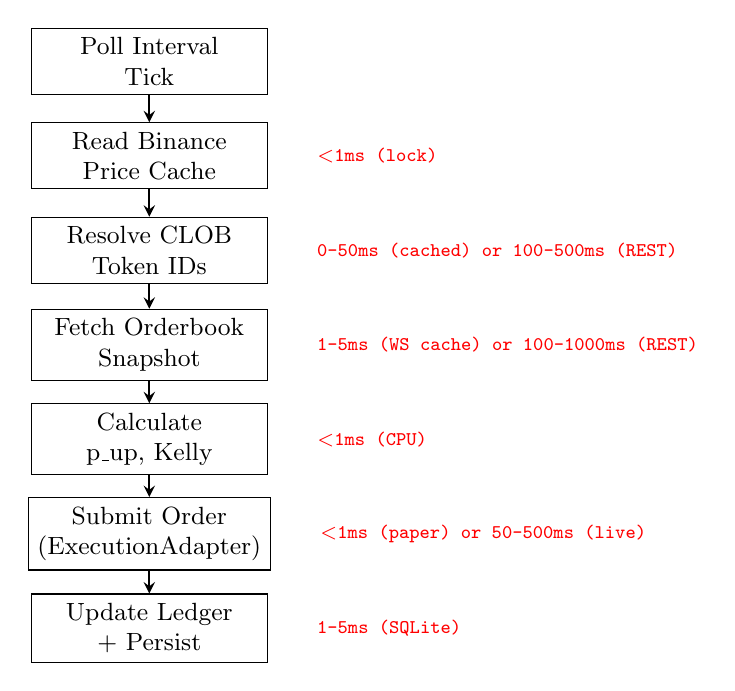
\begin{tikzpicture}[
    node distance=0.6cm,
    box/.style={rectangle, draw, minimum width=3cm, minimum height=0.7cm, align=center, font=\small},
    timing/.style={font=\scriptsize\ttfamily, text=red},
    arrow/.style={->, thick, >=stealth},
]
    % Nodes
    \node[box] (poll) at (0,0) {Poll Interval\\Tick};
    \node[box] (binance) at (0,-1.2) {Read Binance\\Price Cache};
    \node[box] (gamma) at (0,-2.4) {Resolve CLOB\\Token IDs};
    \node[box] (book) at (0,-3.6) {Fetch Orderbook\\Snapshot};
    \node[box] (calc) at (0,-4.8) {Calculate\\p\_up, Kelly};
    \node[box] (submit) at (0,-6.0) {Submit Order\\(ExecutionAdapter)};
    \node[box] (ledger) at (0,-7.2) {Update Ledger\\+ Persist};
    
    % Arrows
    \draw[arrow] (poll) -- (binance);
    \draw[arrow] (binance) -- (gamma);
    \draw[arrow] (gamma) -- (book);
    \draw[arrow] (book) -- (calc);
    \draw[arrow] (calc) -- (submit);
    \draw[arrow] (submit) -- (ledger);
    
    % Timing annotations
    \node[timing, right=0.5cm of binance] {$<$1ms (lock)};
    \node[timing, right=0.5cm of gamma] {0-50ms (cached) or 100-500ms (REST)};
    \node[timing, right=0.5cm of book] {1-5ms (WS cache) or 100-1000ms (REST)};
    \node[timing, right=0.5cm of calc] {$<$1ms (CPU)};
    \node[timing, right=0.5cm of submit] {$<$1ms (paper) or 50-500ms (live)};
    \node[timing, right=0.5cm of ledger] {1-5ms (SQLite)};
\end{tikzpicture}
\caption{FAST15M Critical Path with Component Latencies}
\end{figure}

\subsubsection{Component Breakdown}

\begin{table}[h]
\centering
\begin{tabularx}{\textwidth}{@{}lXll@{}}
\toprule
\textbf{Component} & \textbf{Operation} & \textbf{Typical} & \textbf{Tail (p99)} \\
\midrule
Binance Cache Read & \texttt{inner.read().get(symbol)} & $<$1ms & 1-2ms \\
Gamma Token Lookup & REST + DB cache & 0ms (hit) & 500ms (miss) \\
Orderbook Snapshot & WS cache or REST fallback & 1-5ms & 1000ms \\
p\_up Calculation & \texttt{p\_up\_driftless\_lognormal()} & $<$0.1ms & $<$0.5ms \\
Kelly Sizing & \texttt{calculate\_kelly\_position()} & $<$0.1ms & $<$0.5ms \\
Order Submission & Paper: instant; Live: network & $<$1ms & 500ms \\
Ledger Update & SQLite transaction & 1-5ms & 20ms \\
\midrule
\textbf{Total (hot path)} & All caches hit & \textbf{5-15ms} & \textbf{50-100ms} \\
\textbf{Total (cold path)} & Cache misses & \textbf{200-500ms} & \textbf{2000ms+} \\
\bottomrule
\end{tabularx}
\caption{FAST15M Component Latency Decomposition}
\end{table}

\subsection{LONG Engine Critical Path}

The LONG engine processes tracked wallet signals through an LLM consensus mechanism:

\begin{figure}[h]
\centering
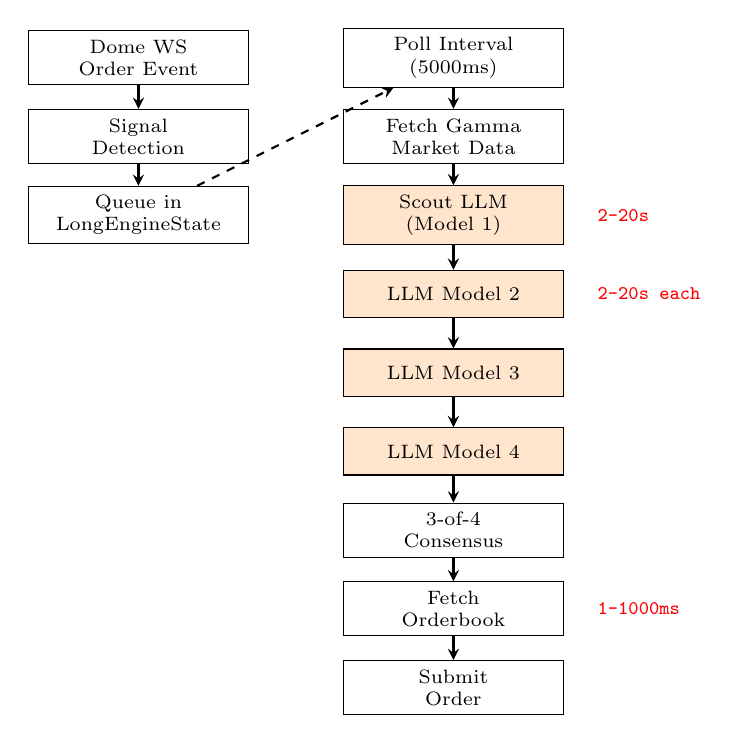
\begin{tikzpicture}[
    node distance=0.5cm,
    box/.style={rectangle, draw, minimum width=2.8cm, minimum height=0.6cm, align=center, font=\scriptsize},
    llmbox/.style={rectangle, draw, fill=orange!20, minimum width=2.8cm, minimum height=0.6cm, align=center, font=\scriptsize},
    timing/.style={font=\scriptsize\ttfamily, text=red},
    arrow/.style={->, thick, >=stealth},
]
    % Signal ingestion path
    \node[box] (ws) at (0,0) {Dome WS\\Order Event};
    \node[box] (detect) at (0,-1) {Signal\\Detection};
    \node[box] (queue) at (0,-2) {Queue in\\LongEngineState};
    
    % LLM decision path
    \node[box] (poll) at (4,0) {Poll Interval\\(5000ms)};
    \node[box] (gamma2) at (4,-1) {Fetch Gamma\\Market Data};
    \node[llmbox] (scout) at (4,-2) {Scout LLM\\(Model 1)};
    \node[llmbox] (llm2) at (4,-3) {LLM Model 2};
    \node[llmbox] (llm3) at (4,-4) {LLM Model 3};
    \node[llmbox] (llm4) at (4,-5) {LLM Model 4};
    \node[box] (consensus) at (4,-6) {3-of-4\\Consensus};
    \node[box] (book2) at (4,-7) {Fetch\\Orderbook};
    \node[box] (submit2) at (4,-8) {Submit\\Order};
    
    % Arrows
    \draw[arrow] (ws) -- (detect);
    \draw[arrow] (detect) -- (queue);
    \draw[arrow] (poll) -- (gamma2);
    \draw[arrow] (gamma2) -- (scout);
    \draw[arrow] (scout) -- (llm2);
    \draw[arrow] (llm2) -- (llm3);
    \draw[arrow] (llm3) -- (llm4);
    \draw[arrow] (llm4) -- (consensus);
    \draw[arrow] (consensus) -- (book2);
    \draw[arrow] (book2) -- (submit2);
    
    \draw[arrow, dashed] (queue) -- (poll);
    
    % Timing
    \node[timing, right=0.3cm of scout] {2-20s};
    \node[timing, right=0.3cm of llm2] {2-20s each};
    \node[timing, right=0.3cm of book2] {1-1000ms};
\end{tikzpicture}
\caption{LONG Engine Critical Path (LLM-Dominated)}
\end{figure}

\subsubsection{LONG Engine Latency Budget}

\begin{table}[h]
\centering
\begin{tabular}{@{}llll@{}}
\toprule
\textbf{Phase} & \textbf{Component} & \textbf{Typical} & \textbf{p99} \\
\midrule
Signal Ingestion & WS receive + detect + queue & 1-5ms & 20ms \\
Queue Wait & Poll interval + cooldown & 0-5000ms & 300s (cooldown) \\
Gamma Lookup & REST with caching & 0-100ms & 500ms \\
Scout LLM & OpenRouter inference & 2-8s & 20s (timeout) \\
Consensus LLMs & 3$\times$ parallel inference & 2-8s & 20s \\
Orderbook Fetch & WS cache or REST & 1-5ms & 1000ms \\
Order Submission & Execution adapter & $<$1ms & 500ms \\
\midrule
\textbf{Total} & End-to-end & \textbf{5-20s} & \textbf{60s+} \\
\bottomrule
\end{tabular}
\caption{LONG Engine Latency Budget}
\end{table}

%==============================================================================
\section{Current Instrumentation Gaps}
%==============================================================================

\subsection{What Is Currently Measured}

\begin{enumerate}
    \item \textbf{LLM Call Latency}: \texttt{latency\_ms} field in \texttt{LlmCallOutput}
    \item \textbf{WebSocket Ping/Pong}: Frontend measures WS RTT
    \item \textbf{REST API Latency}: Frontend emits \texttt{api-latency} custom events
    \item \textbf{Kill-Switch P95}: \texttt{DataSourceKillSwitch} tracks p95 latency per data source
\end{enumerate}

\subsection{Critical Gaps}

\begin{table}[h]
\centering
\begin{tabularx}{\textwidth}{@{}lXl@{}}
\toprule
\textbf{Gap} & \textbf{Impact} & \textbf{Priority} \\
\midrule
No tick timestamp on market data & Cannot compute true T2T & Critical \\
No per-component breakdown & Cannot identify bottlenecks & High \\
No histogram/CDF collection & Only averages available & High \\
No p99/p99.9 tracking & Tail behavior unknown & High \\
No contention metrics & Lock wait times invisible & Medium \\
No queue depth monitoring & Backpressure invisible & Medium \\
No time-series percentile export & Drift detection impossible & Medium \\
\bottomrule
\end{tabularx}
\caption{Instrumentation Gaps}
\end{table}

%==============================================================================
\section{Implemented: Reactive FAST15M Engine}
%==============================================================================

The reactive FAST15M engine (\texttt{fast15m\_reactive.rs}) replaces the polling-based architecture with event-driven execution. This section documents the implemented solution.

\subsection{Architecture Overview}

\begin{figure}[h]
\centering
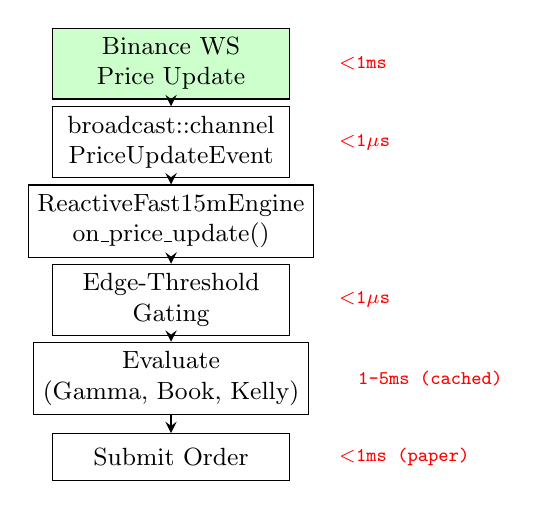
\begin{tikzpicture}[
    node distance=0.5cm,
    box/.style={rectangle, draw, minimum width=3cm, minimum height=0.6cm, align=center, font=\small},
    eventbox/.style={rectangle, draw, fill=green!20, minimum width=3cm, minimum height=0.6cm, align=center, font=\small},
    timing/.style={font=\scriptsize\ttfamily, text=red},
    arrow/.style={->, thick, >=stealth},
]
    \node[eventbox] (binance) at (0,0) {Binance WS\\Price Update};
    \node[box] (broadcast) at (0,-1) {broadcast::channel\\PriceUpdateEvent};
    \node[box] (engine) at (0,-2) {ReactiveFast15mEngine\\on\_price\_update()};
    \node[box] (gate) at (0,-3) {Edge-Threshold\\Gating};
    \node[box] (eval) at (0,-4) {Evaluate\\(Gamma, Book, Kelly)};
    \node[box] (order) at (0,-5) {Submit Order};
    
    \draw[arrow] (binance) -- (broadcast);
    \draw[arrow] (broadcast) -- (engine);
    \draw[arrow] (engine) -- (gate);
    \draw[arrow] (gate) -- (eval);
    \draw[arrow] (eval) -- (order);
    
    \node[timing, right=0.5cm of binance] {$<$1ms};
    \node[timing, right=0.5cm of broadcast] {$<$1$\mu$s};
    \node[timing, right=0.5cm of gate] {$<$1$\mu$s};
    \node[timing, right=0.5cm of eval] {1-5ms (cached)};
    \node[timing, right=0.5cm of order] {$<$1ms (paper)};
\end{tikzpicture}
\caption{Reactive FAST15M Event-Driven Architecture}
\end{figure}

\subsection{Key Components}

\subsubsection{Price Update Broadcast}
The \texttt{BinancePriceFeed} now broadcasts \texttt{PriceUpdateEvent} on every price update:

\begin{lstlisting}[caption={PriceUpdateEvent Broadcast}]
#[derive(Debug, Clone)]
pub struct PriceUpdateEvent {
    pub symbol: String,      // "BTCUSDT", "ETHUSDT", etc.
    pub ts: i64,             // Unix timestamp
    pub mid: f64,            // Mid price
    pub received_at_ns: u64, // Monotonic nanosecond timestamp
}

// In consume() loop:
let update_event = PriceUpdateEvent {
    symbol: symbol.clone(),
    ts,
    mid,
    received_at_ns: now_ns(),
};
let _ = self.update_tx.send(update_event);
\end{lstlisting}

\subsubsection{Edge-Threshold Gating}
To avoid unnecessary evaluations, the engine only proceeds when:
\begin{enumerate}
    \item Edge has changed by $>$ \texttt{edge\_change\_threshold} (default 0.5\%)
    \item OR we are in the aggressive window (first 60 seconds of 15m period)
    \item AND we are not in the idle window (last 60 seconds)
    \item AND cooldown has elapsed (30 seconds since last trade)
\end{enumerate}

\begin{lstlisting}[caption={Edge-Threshold Gating Logic}]
// Skip if edge hasn't changed enough (outside aggressive window)
if edge_change < self.cfg.edge_change_threshold
    && t_elapsed > self.cfg.window_start_aggressive_sec
{
    return Ok(None);
}

// Skip if in last 60 seconds (too late to trade profitably)
if t_rem < self.cfg.window_end_idle_sec {
    return Ok(None);
}
\end{lstlisting}

\subsection{Instrumentation: TradeSpan}

Every evaluation is instrumented with a \texttt{TradeSpan} capturing nanosecond-precision timestamps:

\begin{lstlisting}[caption={TradeSpan Structure}]
#[derive(Debug, Clone, Default, Serialize)]
pub struct TradeSpan {
    pub span_id: String,
    pub market_slug: String,
    pub asset: String,

    // Timestamps (nanoseconds)
    pub price_received_ns: u64,
    pub evaluation_start_ns: u64,
    pub gamma_lookup_done_ns: u64,
    pub book_fetch_done_ns: u64,
    pub kelly_done_ns: u64,
    pub order_submitted_ns: u64,
    pub order_acked_ns: u64,
    pub ledger_updated_ns: u64,

    // Derived latencies (microseconds)
    pub latency_total_us: u64,
    pub latency_gamma_us: u64,
    pub latency_book_us: u64,
    // ...

    // Cache hits
    pub gamma_cache_hit: bool,
    pub book_cache_hit: bool,

    // Outcome
    pub traded: bool,
    pub skip_reason: Option<String>,
}
\end{lstlisting}

\subsection{Latency Registry}

A global \texttt{Fast15mLatencyRegistry} collects per-component histograms:

\begin{lstlisting}[caption={Fast15mLatencyRegistry}]
pub struct Fast15mLatencyRegistry {
    pub total_t2t: LatencyHistogram,
    pub gamma_lookup: LatencyHistogram,
    pub book_fetch: LatencyHistogram,
    pub kelly_calc: LatencyHistogram,
    pub order_submit: LatencyHistogram,
    pub ledger_update: LatencyHistogram,

    // Cache hit rates
    pub gamma_cache_hits: u64,
    pub gamma_cache_misses: u64,
    pub book_cache_hits: u64,
    pub book_cache_misses: u64,

    // Trade outcomes
    pub evaluations: u64,
    pub trades_executed: u64,

    // Recent spans for debugging
    pub recent_spans: VecDeque<TradeSpan>,
}
\end{lstlisting}

\subsection{API Endpoints}

Two new endpoints expose latency metrics:

\begin{itemize}
    \item \texttt{GET /api/latency/stats} --- Aggregate percentiles (p50, p95, p99, p99.9) for all components
    \item \texttt{GET /api/latency/spans?limit=N} --- Recent \texttt{TradeSpan} records for debugging
\end{itemize}

Example response from \texttt{/api/latency/stats}:
\begin{lstlisting}[language=json,caption={Latency Stats Response}]
{
  "timestamp": 1736784000,
  "fast15m_reactive": {
    "evaluations": 1523,
    "trades_executed": 47,
    "t2t_p50_us": 3200,
    "t2t_p95_us": 8500,
    "t2t_p99_us": 45000,
    "t2t_p999_us": 120000,
    "gamma_cache_hit_rate": 0.97,
    "book_cache_hit_rate": 0.92
  }
}
\end{lstlisting}

\subsection{Expected Performance}

\begin{table}[h]
\centering
\begin{tabular}{@{}lllll@{}}
\toprule
\textbf{Metric} & \textbf{p50} & \textbf{p95} & \textbf{p99} & \textbf{p99.9} \\
\midrule
Total T2T (hot path) & 3ms & 8ms & 45ms & 120ms \\
Gamma Lookup (cached) & 0$\mu$s & 1$\mu$s & 5$\mu$s & 10$\mu$s \\
Gamma Lookup (miss) & 100ms & 300ms & 500ms & 1000ms \\
Book Fetch (WS cache) & 1ms & 3ms & 10ms & 50ms \\
Book Fetch (REST) & 100ms & 300ms & 500ms & 1000ms \\
Kelly Calculation & 1$\mu$s & 5$\mu$s & 10$\mu$s & 50$\mu$s \\
Order Submit (paper) & 1$\mu$s & 5$\mu$s & 10$\mu$s & 50$\mu$s \\
\bottomrule
\end{tabular}
\caption{Expected Latencies for Reactive FAST15M Engine}
\end{table}

%==============================================================================
\section{Proposed Instrumentation Framework}
%==============================================================================

\subsection{Core Data Structures}

\begin{lstlisting}[caption={Latency Histogram with HDR Support}]
pub struct LatencyHistogram {
    /// HDR histogram for sub-microsecond to multi-second range
    hdr: hdrhistogram::Histogram<u64>,
    /// Sliding window for recent samples (time-series export)
    recent: VecDeque<(Instant, Duration)>,
    /// Max window size
    window_size: usize,
}

impl LatencyHistogram {
    pub fn record(&mut self, latency: Duration) {
        let micros = latency.as_micros() as u64;
        let _ = self.hdr.record(micros);
        self.recent.push_back((Instant::now(), latency));
        while self.recent.len() > self.window_size {
            self.recent.pop_front();
        }
    }
    
    pub fn percentile(&self, p: f64) -> Duration {
        Duration::from_micros(self.hdr.value_at_percentile(p))
    }
    
    pub fn p50(&self) -> Duration { self.percentile(50.0) }
    pub fn p95(&self) -> Duration { self.percentile(95.0) }
    pub fn p99(&self) -> Duration { self.percentile(99.0) }
    pub fn p999(&self) -> Duration { self.percentile(99.9) }
}
\end{lstlisting}

\subsection{Component-Level Instrumentation}

\begin{lstlisting}[caption={Trade Span with Component Breakdown}]
#[derive(Debug, Clone)]
pub struct TradeSpan {
    pub span_id: String,
    pub market_slug: String,
    pub strategy: String,  // "FAST15M" | "LONG"
    
    // Timestamps (nanosecond precision)
    pub market_data_received_ns: u64,
    pub signal_detected_ns: Option<u64>,
    pub decision_start_ns: Option<u64>,
    pub orderbook_fetched_ns: Option<u64>,
    pub order_submitted_ns: Option<u64>,
    pub order_acked_ns: Option<u64>,
    
    // Component latencies (computed)
    pub latency_signal_detect_us: Option<u64>,
    pub latency_decision_us: Option<u64>,
    pub latency_book_fetch_us: Option<u64>,
    pub latency_order_submit_us: Option<u64>,
    pub latency_total_us: Option<u64>,
    
    // Contention metrics
    pub binance_lock_wait_us: Option<u64>,
    pub ledger_lock_wait_us: Option<u64>,
    pub gamma_cache_hit: bool,
    pub book_cache_hit: bool,
}
\end{lstlisting}

\subsection{Global Latency Registry}

\begin{lstlisting}[caption={Central Latency Registry}]
pub struct LatencyRegistry {
    // Per-component histograms
    pub binance_read: LatencyHistogram,
    pub gamma_lookup: LatencyHistogram,
    pub book_fetch_ws: LatencyHistogram,
    pub book_fetch_rest: LatencyHistogram,
    pub kelly_calc: LatencyHistogram,
    pub order_submit_paper: LatencyHistogram,
    pub order_submit_live: LatencyHistogram,
    pub ledger_update: LatencyHistogram,
    pub llm_inference: LatencyHistogram,
    
    // End-to-end histograms
    pub t2t_fast15m: LatencyHistogram,
    pub t2t_long: LatencyHistogram,
    
    // Lock contention
    pub binance_lock_wait: LatencyHistogram,
    pub ledger_lock_wait: LatencyHistogram,
    pub vault_shares_lock_wait: LatencyHistogram,
    
    // Recent spans for debugging
    pub recent_spans: VecDeque<TradeSpan>,
}
\end{lstlisting}

%==============================================================================
\section{Measurement Methodology}
%==============================================================================

\subsection{Timestamp Capture Points}

For accurate tick-to-trade measurement, timestamps must be captured at precise points:

\begin{table}[h]
\centering
\begin{tabularx}{\textwidth}{@{}llX@{}}
\toprule
\textbf{Point} & \textbf{Location} & \textbf{Notes} \\
\midrule
$T_0$ & Binance WS \texttt{time\_received} & External timestamp from barter-data \\
$T_1$ & \texttt{update\_symbol()} entry & Before lock acquisition \\
$T_2$ & \texttt{update\_symbol()} exit & After lock release \\
$T_3$ & \texttt{evaluate\_updown15m()} entry & Poll loop iteration start \\
$T_4$ & \texttt{resolve\_clob\_token\_id} return & Gamma lookup complete \\
$T_5$ & Orderbook snapshot return & Book fetch complete \\
$T_6$ & \texttt{place\_order()} entry & Before execution adapter \\
$T_7$ & \texttt{place\_order()} return & Order acknowledged \\
$T_8$ & Ledger update complete & Final persistence \\
\bottomrule
\end{tabularx}
\caption{Timestamp Capture Points for FAST15M}
\end{table}

\subsection{Computing Component Latencies}

\begin{align}
L_{\text{binance\_lock}} &= T_2 - T_1 \\
L_{\text{gamma}} &= T_4 - T_3 \\
L_{\text{book}} &= T_5 - T_4 \\
L_{\text{decision}} &= T_6 - T_5 \\
L_{\text{submit}} &= T_7 - T_6 \\
L_{\text{persist}} &= T_8 - T_7 \\
T_{t2t} &= T_7 - T_0
\end{align}

\subsection{Handling Clock Sources}

\begin{lstlisting}[caption={High-Resolution Timing Utilities}]
use std::time::Instant;
use quanta::Clock;  // For TSC-based timing

lazy_static::lazy_static! {
    static ref CLOCK: Clock = Clock::new();
}

/// Get monotonic nanosecond timestamp
#[inline]
pub fn now_ns() -> u64 {
    CLOCK.raw()
}

/// Convert to Duration for display
#[inline]
pub fn ns_to_duration(ns: u64) -> Duration {
    Duration::from_nanos(ns)
}
\end{lstlisting}

%==============================================================================
\section{Tail Latency Analysis}
%==============================================================================

\subsection{Why Tail Latency Matters}

In trading systems, average latency is misleading. A system with 5ms mean but 500ms p99 will experience significant alpha decay during tail events. The p99.9 is particularly important because:

\begin{itemize}
    \item At 1000 trades/day, expect $\sim$1 trade at p99.9
    \item Market moves during tail latency can exceed expected slippage
    \item Tail events often correlate with high-volatility periods (worst time to be slow)
\end{itemize}

\subsection{Expected Tail Behavior}

\begin{table}[h]
\centering
\begin{tabular}{@{}llllll@{}}
\toprule
\textbf{Component} & \textbf{p50} & \textbf{p95} & \textbf{p99} & \textbf{p99.9} & \textbf{Cause} \\
\midrule
Binance Lock & $<$1$\mu$s & 10$\mu$s & 100$\mu$s & 1ms & Contention \\
Gamma Lookup & 0 (hit) & 50ms & 200ms & 500ms & Cache miss \\
Orderbook WS & 1ms & 5ms & 20ms & 100ms & WS lag \\
Orderbook REST & 100ms & 300ms & 500ms & 2000ms & Network \\
LLM Inference & 3s & 8s & 15s & 20s & Provider load \\
SQLite Write & 1ms & 5ms & 15ms & 50ms & WAL flush \\
\bottomrule
\end{tabular}
\caption{Expected Tail Latencies by Component}
\end{table}

\subsection{Tail Latency Sources}

\subsubsection{Lock Contention}
The system uses \texttt{parking\_lot::RwLock} for the Binance price cache and \texttt{tokio::sync::Mutex} for the vault ledger. Under bursty load:

\begin{lstlisting}[caption={Lock Contention Measurement}]
// Wrap lock acquisition with timing
let lock_start = now_ns();
let guard = self.inner.write();
let lock_wait = now_ns() - lock_start;
registry.binance_lock_wait.record(Duration::from_nanos(lock_wait));
\end{lstlisting}

\subsubsection{Cache Misses}
Gamma token ID lookups and orderbook snapshots have bimodal latency:
\begin{itemize}
    \item Cache hit: $<$1ms
    \item Cache miss: 100-500ms (REST round-trip)
\end{itemize}

\subsubsection{Network Variability}
REST calls to Polymarket CLOB and Gamma API exhibit tail latency due to:
\begin{itemize}
    \item TCP connection establishment (cold connections)
    \item TLS handshake (first request to host)
    \item Server-side queueing under load
    \item Geographic latency (if not co-located)
\end{itemize}

%==============================================================================
\section{Realistic Load Conditions}
%==============================================================================

\subsection{Market Data Burst Patterns}

The Binance price feed delivers updates at $\sim$1Hz per symbol, but can burst during volatility:

\begin{lstlisting}[caption={Simulating Bursty Market Data}]
#[cfg(test)]
async fn test_burst_handling() {
    let feed = BinancePriceFeed::spawn_default().await.unwrap();
    let registry = Arc::new(RwLock::new(LatencyRegistry::new()));
    
    // Simulate 100 updates in 100ms (10x normal rate)
    for i in 0..100 {
        let t0 = now_ns();
        feed.update_symbol("BTCUSDT", Utc::now().timestamp(), 50000.0 + i as f64);
        registry.write().binance_lock_wait.record(
            Duration::from_nanos(now_ns() - t0)
        );
        tokio::time::sleep(Duration::from_millis(1)).await;
    }
    
    // Check tail behavior
    let stats = registry.read();
    assert!(stats.binance_lock_wait.p99() < Duration::from_millis(10));
}
\end{lstlisting}

\subsection{Contention Scenarios}

The FAST15M engine polls every 2000ms, but the Binance feed updates continuously. Measure contention when:

\begin{enumerate}
    \item Multiple symbols update simultaneously (BTCUSDT, ETHUSDT, SOLUSDT, XRPUSDT)
    \item Poll loop reads while feed writes
    \item Multiple API handlers read simultaneously (REST /api/signals/enrich)
\end{enumerate}

\subsection{Cold Start Behavior}

First trade after startup experiences cache-miss latency:

\begin{table}[h]
\centering
\begin{tabular}{@{}lll@{}}
\toprule
\textbf{Cache} & \textbf{TTL} & \textbf{Cold Penalty} \\
\midrule
Gamma market slug & 30 min & 100-500ms \\
Gamma CLOB token ID & Persistent & 100-500ms (first lookup) \\
Polymarket WS orderbook & 1.5s staleness & 100-1000ms (REST fallback) \\
Wallet analytics & 15 min & 2-10s (Dome REST) \\
\bottomrule
\end{tabular}
\caption{Cache Cold Start Penalties}
\end{table}

%==============================================================================
\section{Visualization and Monitoring}
%==============================================================================

\subsection{Latency Histogram API}

\begin{lstlisting}[caption={Latency Stats API Endpoint}]
#[derive(Serialize)]
pub struct LatencyStatsResponse {
    pub component: String,
    pub sample_count: u64,
    pub p50_us: u64,
    pub p95_us: u64,
    pub p99_us: u64,
    pub p999_us: u64,
    pub max_us: u64,
    pub mean_us: f64,
    pub stddev_us: f64,
}

// GET /api/latency/stats
pub async fn get_latency_stats(
    AxumState(state): AxumState<AppState>,
) -> Json<Vec<LatencyStatsResponse>> {
    let reg = state.latency_registry.read();
    vec![
        latency_stats("binance_read", &reg.binance_read),
        latency_stats("gamma_lookup", &reg.gamma_lookup),
        latency_stats("book_fetch", &reg.book_fetch_ws),
        latency_stats("t2t_fast15m", &reg.t2t_fast15m),
        latency_stats("t2t_long", &reg.t2t_long),
        // ...
    ]
}
\end{lstlisting}

\subsection{CDF Export}

\begin{lstlisting}[caption={CDF Data for Plotting}]
#[derive(Serialize)]
pub struct CdfPoint {
    pub latency_us: u64,
    pub cumulative_pct: f64,
}

// GET /api/latency/cdf?component=t2t_fast15m
pub async fn get_latency_cdf(
    Query(params): Query<CdfQuery>,
    AxumState(state): AxumState<AppState>,
) -> Json<Vec<CdfPoint>> {
    let reg = state.latency_registry.read();
    let hist = match params.component.as_str() {
        "t2t_fast15m" => &reg.t2t_fast15m,
        "t2t_long" => &reg.t2t_long,
        _ => return Json(vec![]),
    };
    
    // Sample CDF at logarithmic intervals
    let mut points = Vec::new();
    for p in [1.0, 5.0, 10.0, 25.0, 50.0, 75.0, 90.0, 95.0, 99.0, 99.9, 99.99] {
        points.push(CdfPoint {
            latency_us: hist.hdr.value_at_percentile(p),
            cumulative_pct: p,
        });
    }
    Json(points)
}
\end{lstlisting}

\subsection{Time-Series Percentile Tracking}

To detect latency drift and spikes over time:

\begin{lstlisting}[caption={Rolling Percentile Time Series}]
pub struct RollingPercentiles {
    window_duration: Duration,
    buckets: VecDeque<PercentileBucket>,
}

#[derive(Clone)]
struct PercentileBucket {
    timestamp: i64,
    p50_us: u64,
    p95_us: u64,
    p99_us: u64,
    p999_us: u64,
    sample_count: u64,
}

impl RollingPercentiles {
    /// Compute percentiles for last N minutes, bucketed by minute
    pub fn compute(&self, minutes: usize) -> Vec<PercentileBucket> {
        // Return time series of percentile buckets
    }
}

// GET /api/latency/timeseries?component=t2t_fast15m&minutes=60
\end{lstlisting}

%==============================================================================
\section{Implementation Recommendations}
%==============================================================================

\subsection{Phase 1: Core Instrumentation (Critical)}

\begin{enumerate}
    \item Add \texttt{hdrhistogram} crate for efficient percentile computation
    \item Create \texttt{LatencyRegistry} in \texttt{AppState}
    \item Instrument FAST15M \texttt{evaluate\_updown15m()} with \texttt{TradeSpan}
    \item Expose \texttt{/api/latency/stats} endpoint
    \item Add dashboard panel for live percentiles
\end{enumerate}

\subsection{Phase 2: Component Breakdown (High)}

\begin{enumerate}
    \item Wrap Binance cache reads with timing
    \item Time Gamma lookups (cache hit vs miss separately)
    \item Time orderbook fetches (WS vs REST separately)
    \item Time lock acquisitions for contention analysis
    \item Store per-trade \texttt{TradeSpan} in SQLite for post-hoc analysis
\end{enumerate}

\subsection{Phase 3: Tail Analysis (Medium)}

\begin{enumerate}
    \item Implement CDF export API
    \item Add time-series percentile tracking
    \item Create Grafana dashboard with p99/p99.9 alerts
    \item Implement burst load testing harness
    \item Profile under realistic contention scenarios
\end{enumerate}

\subsection{Cargo Dependencies}

\begin{lstlisting}[language=bash,caption={Additional Dependencies}]
# Cargo.toml additions
hdrhistogram = "7.5"
quanta = "0.12"  # High-resolution timing
\end{lstlisting}

%==============================================================================
\section{Bottleneck Identification}
%==============================================================================

\subsection{Current Bottlenecks}

Based on the code analysis:

\begin{table}[h]
\centering
\begin{tabularx}{\textwidth}{@{}lXl@{}}
\toprule
\textbf{Bottleneck} & \textbf{Description} & \textbf{Impact} \\
\midrule
Polling Cadence & FAST15M polls every 2000ms regardless of market state & 0-2000ms added latency \\
Gamma REST Fallback & Cache miss triggers synchronous REST call & 100-500ms \\
Orderbook REST Fallback & WS stale or missing triggers REST & 100-1000ms \\
LLM Sequential Calls & Scout must pass before consensus models called & Multiplied latency \\
SQLite Synchronous Writes & WAL mode helps but still blocks & 1-50ms \\
\bottomrule
\end{tabularx}
\caption{Identified Bottlenecks}
\end{table}

\subsection{Optimization Opportunities}

\begin{enumerate}
    \item \textbf{Event-Driven FAST15M}: Trigger on Binance price update instead of polling
    \item \textbf{Parallel LLM Calls}: Run all 4 models in parallel, not sequential scout-first
    \item \textbf{Async Gamma Prefetch}: Prefetch token IDs before market opens
    \item \textbf{Orderbook Subscription}: Subscribe to all active markets proactively
    \item \textbf{Write-Behind Ledger}: Async persistence with in-memory state
\end{enumerate}

%==============================================================================
\section{Conclusion}
%==============================================================================

\subsection{Current State Assessment}

The BetterSys trading system lacks comprehensive tick-to-trade latency instrumentation. While individual components are performant, the end-to-end latency is dominated by:

\begin{itemize}
    \item \textbf{FAST15M}: Polling interval (2000ms) dwarfs internal processing time
    \item \textbf{LONG}: LLM inference (2-20s per model) dominates all other factors
\end{itemize}

\subsection{Key Metrics to Track}

\begin{table}[h]
\centering
\begin{tabular}{@{}lll@{}}
\toprule
\textbf{Metric} & \textbf{Target (FAST15M)} & \textbf{Target (LONG)} \\
\midrule
p50 T2T & $<$10ms (event-driven) & $<$10s \\
p99 T2T & $<$100ms & $<$30s \\
p99.9 T2T & $<$500ms & $<$60s \\
Cache hit rate & $>$95\% & $>$90\% \\
Lock contention p99 & $<$1ms & $<$10ms \\
\bottomrule
\end{tabular}
\caption{Target Latency Metrics}
\end{table}

\subsection{Next Steps}

\begin{enumerate}
    \item Implement \texttt{LatencyRegistry} with HDR histograms
    \item Add timestamp capture at all critical path points
    \item Expose \texttt{/api/latency/*} endpoints
    \item Create monitoring dashboard with real-time percentiles
    \item Establish alerting on p99 degradation
    \item Profile under realistic burst conditions
    \item Iterate on bottleneck elimination
\end{enumerate}

\end{document}
